%------------------------------------------------------
%Author             : Daniel Schembri, Jonathan Schwarz
%University         : Pforzheim University
%Date of last edit  : Wed, 03 Sep 2014 14:12:16 +0200
%Filename           : multithreading_with_posix_pthreads.tex
%------------------------------------------------------

\documentclass[10pt,a4paper,DIV=11]{scrreprt}

%British English
\usepackage[UKenglish]{babel}
%utf8
\usepackage[utf8]{inputenc}

%Multicolumn lists
\usepackage{multicol}

%pseudo-code
\usepackage[boxruled,vlined]{algorithm2e}

%for source code listings
\usepackage{listings}

\usepackage[table]{xcolor}

%tikz
\usepackage{tikz}
\usetikzlibrary{arrows,positioning,fit}

%plots
\usepackage{pgfplots}

%blocks - used by tikz-uml, included before
\pgfdeclarelayer{background}
\pgfdeclarelayer{foreground}
\pgfsetlayers{background,main,foreground}

%<,> in tikz-uml
\usepackage[T1]{fontenc}
\usepackage{tikz-uml}

%subfigure
\usepackage{graphicx}
\usepackage{subfigure}

%prevent figure from floating pictures
\usepackage{float}

%footer & header
\usepackage{fancyhdr}

%push footer down
\usepackage[bottom]{footmisc}

%footer & header
\pagestyle{fancy}
%clean footer & header
\fancyhf{}

%bibtex
\usepackage[square,numbers]{natbib}
\usepackage{gensymb}

%equation
\usepackage[tbtags]{amsmath}
\usepackage{amssymb} 

%table of contents with hyperlinks
%always include as last package
\usepackage{hyperref}

%===========================TITLE PAGE=======================================

%university logo
\titlehead
{
    
\includegraphics[width=0.20\textwidth]{files/hspflogo.pdf}\\

    Pforzheim University\\
    School of Engineering\\
}

\subject{Project work}
	
\title
{
    Simulation and evolutionary training of object collecting agents\\
}

\author
{
    by \textbf{Daniel Schembri} - matriculation number: 310026
}
\date
{
    Winter term 2013/2014
}
%\today{}}

\publishers
{
    Examiner: Prof. Dr. Richard Alznauer\\
    Supervisor: Dr. Christoph Ussfeller
}


%=========================================GLOBAL SETTINGS=========================================

%footer &header

%\fancyfoot[L]{\textbf{Multi-Threading mit POSIX-pThreads}}
\fancyhead[R]{Page \thepage}
%\fancyhead[L]{\thechapter}

%chapter number and title
\fancyhead[L]{\nouppercase{\leftmark}}
%line
%\renewcommand{\footrulewidth}{0.5 pt}
\usepackage{lmodern}
\addtokomafont{sectioning}{\rmfamily}
\setlength{\parindent}{0mm}

%colour definitions
\definecolor{dkgreen}{rgb}{0,0.6,0}
\definecolor{gray}{rgb}{0.7,0.7,0.7}
%medium gray
\definecolor{mgray}{gray}{0.80}
%light gray
\definecolor{lgray}{gray}{0.97}

%hyperlink settings
%frame around hyperlinks
\hypersetup
{
    colorlinks = false,
    linkcolor = black,
    hypertexnames = false,
    citecolor = green
}

%listing settings
\lstset
{ 
    language=C++,                
    basicstyle=\footnotesize\ttfamily,           
    numbers=left,
    stepnumber=5,    
    firstnumber=1,
    numberfirstline=true                 
    numberstyle=\color{black},                 
    numbersep=5pt,                 
    backgroundcolor=\color{white},      
    showspaces=false,             
    showstringspaces=false,         
    showtabs=false,                
    frame=single,                   
    rulecolor=\color{black},       
    tabsize=2,                     
    captionpos=b,                   
    breaklines=true,                
    breakatwhitespace=false,       
    title=\lstname,                    
    keywordstyle=\color{blue},          
    commentstyle=\color{dkgreen}, 
    identifierstyle=\color{black},      
    stringstyle=\color{purple},      
    escapeinside={\%*}{*)},      
    morekeywords={*,...},            
    deletekeywords={...}             
}

\setcounter{tocdepth}{4}  %a deeper contentsmenue
%=====================================DOCUMENT START=========================
\begin{document}

\tikzstyle{line}=[draw]
\tikzstyle{arrow}=[draw, -latex] 

%\renewcommand*\contentsname{Content}
%\renewcommand*\listtablename{Tables}
%\renewcommand*\listfigurename{Figures}
%\renewcommand*\bibname{Literature references}

\maketitle
\thispagestyle{empty}
\newpage
{\large\tableofcontents}
\newpage

% Ideas for the documentation 
% -> Robots playing football
% -> 
% 
%
%
%
%



\chapter{Introduction}
Intelligent systems are widely used, like in robotics.
The motivation to write this projectwork was
to find out basically, how an intelligent system can be created by simple algorithms (rules) and compare them with 'classical' solutions. Therefore a simple task was to let agents collect objects in a virtual environment.



In this project neural networks of the second type are used, because the main interest lies in finding a good mathematical solution.

2-dimensional because its easier to see.

\section{State of the art}

\section{Artificial intelligence}
Today there is no exact definition of what intelligence is.
In general there are certain categories focusing different points of view to describe it.


\chapter{The concept of agents}
An agent is a programm that interacts self-sufficent depending on the actual state. It has, in general sensors, a processing logic and actuators. The input data will be processed to behave in the desired way. In the simplest case this could be a table containing the required output to every possible input. In this project the concept of agents is used to compare with neural networks.

Most agents are found in the world wide web. For example webcrawlers, search-engines and bots are well known.


\begin{center}
	\begin{figure}[H]
		\centering
		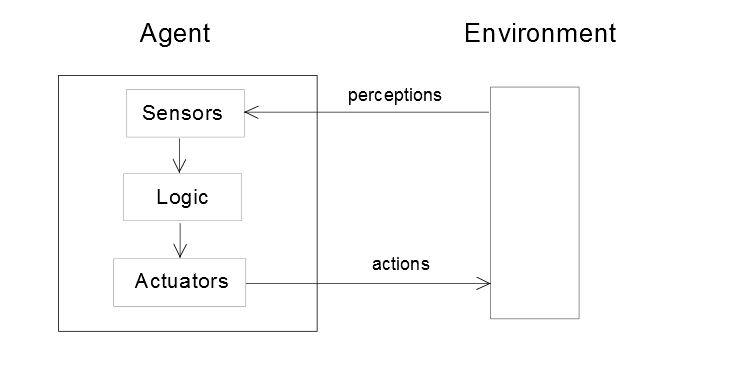
\includegraphics[width=1.0\textwidth,scale=1]{files/agent.png}  
		\caption{General structure of an agent (oriented on \cite{ki-book} )} 
		\label{fig:agent}
	\end{figure}
\end{center}



\subsection{Rationality}
An agent creates a sequence of actions. These actions causes a sequence of states in the corresponding environment. Every sequence of states can be rated. The agent is called rational if it can maximize its score, considering its sequence of perceptions and its previous knowledge of the problem. Its important to distinguish rationality and perfection. An agent never will be perfectly solving a problem. Its unrealistic to expect the best possible solution for a problem in partitial observable environment. It can solve the problem as it can be expected by the given perceptions. The agent can't predict randomly events.

To achieve rationality the following topics have to be considered: \\

\fbox{
	\begin{minipage}{15cm}
		\begin{itemize} 
			\item A sufficient previous knowledge of the problem.
			\item A good rating of the resulting state sequence of the environment.
			\item The perception sequence.
			\item The possible actions the agent can execute.
		\end{itemize}
	\end{minipage}
}   \\

\subsubsection{Learning}
It is important for the agent to get further knowledge by its perceptions. Therefore the agent has to make some actions to explore the world, if he acts in a unknown environment.
An agent who doesn't learn can most likely not solve a problem if the environment changes.
In nature animals are equipped with reflex actions to survive long enough to learn to handle with their environment.

\section{Types of agents}

TODO: Describe the agent program.
TODO: Prove the english topics in the original book!

\subsection{Simple reflex agent}
The simplest type of an agent is the reflex based agent.
This agent ignores the sequence of perception and just acts on the sensordata it actually gets. This type of agent can be used for simple tasks. The benefits are the fast implementation and a drastically reduced state space.
The disadvantages lies in the simplicity. This agent has no memory and therefore doesn't include past states in his decisions. If the present state of the environment doesn't provide enough information or it is just partially observable, the agent could not solve the task.
In partially observebale environment there can occur loops of wrong behaviour. This loops can be overcome if a random action can be chosen.
For best functionality of a simple reflex agent the problem-environment should be fully observable(TODO: note to the next section).
For more complex tasks using the following described agent-types may be a better solution.

\subsection{Model-based reflex agent}
The model-based reflex agent expands the simple reflex agent by a memory. It internally creates a model of the world by past sensor data.
This model is used to predict future states in the environment.
This can be a moving object or changes in the environment made by the agent itself for example.

Internally states of the agent are used to approximate the state of the environment on changes. 
The model is also used to estimate temporaly unobservable parts of the environment.

The model-based reflex agents ability to solve a task reaches its limit, if he has to act in a new environment or other agents acting in the world, too. The internally created model may then not fit anymore.


\subsection{Goal-based agent}
On some tasks it isn't enough to know the correct action on a specified state at the environment, like reflex-based agents do. It can be important for an agent to know the goal behind those actions. This is necessary for a generalization of a problem. For example: For a given route A To B there can be described a sequence of actions an agent has to execute. In general to get from one point to another its more difficult to describe general rules, as other routes may differ a lot. Its therefore too complex to describe all rules in detail. 

The benefit is a agent who can solve complex tasks. The disadvantage is a need of more computing time. For real-time tasks this can be an obstacle.

\subsection{Utility-based agent}
The utility-based agent expands the goal-based agent by the fact, that it can choose between several solutions. Therefore the agent has a rating function to choose the best or at least a good enough solution by several criteria. This rating function can be more complex then computing solutions of the task itself.

The development of such complex agent and corresponding rating algorithms is an own topic of computer science and includes research areas like perception, representation, reasoning and learning.


\subsection{Learning agent}
The complete development of an agent is difficult and time-consuming. Therefore Alan Turing searched in 1950 (TODO: Source Turing) for a way to speed up this process. The concept of the learning agent was created. The learning agent has four components: \\

\fbox{
	\begin{minipage}{15cm}
		\begin{multicols}{2}
			\begin{itemize}
				\item \textbf{Performance element}
				\item \textbf{Learning element}
				\item \textbf{Critic}
				\item \textbf{Problem generator}
			\end{itemize}
		\end{multicols}
	\end{minipage}
}   \\
\\

The \textbf{performance element} is the executive part of the agent. It processes sensor data and makes actions. \\

The \textbf{learning element} is responsible for improvements of the agent. The learning element can contain a decision tree, a neural net, a support vector machine or other learning structures. \\

The \textbf{critic} rates the performance element and tells the learning element how to improve it. \\

A \textbf{problem generator} is used to improve learning by making new experiences. Without the problem generator the agent would make it actions with its learned best actions, but would never try new actions, that may seem uneffective in the first way, but in a long term run may be more effective. \\

The most important part for improvements is the correlation between the \textbf{performance element} and the \textbf{learning element}.





source: Artificial Intelligence Book and www.cs.hs-rm.de/~linn/fachsem0910/anders/Anders.pdf


\section{The task environment}
(TODO: Aufgabenumgebung englsiches Wort)
In the first case its important to preferably define the task completely. The task environment is defined by four categories: \\

\fbox{
	\begin{minipage}{15cm}
		\begin{multicols}{2}
			\begin{itemize} 
				\item \textbf{The performance}
				\item \textbf{The environment}
				\item \textbf{Actuators}
				\item \textbf{Sensors}
			\end{itemize}
		\end{multicols}
	\end{minipage}
}   \\
\\

\textbf{The performance} is defined by the rating the agent can achieve. Therefore \\

\textbf{The environment}
If the sensors allow the agent to get the information of the whole environment, the environment is called \textbf{fully observeable}. The agent therefore can get all relevant information for its actions. Otherwise an environment is classified as \textbf{partially observeable}. This for example can be if the sensors are limited or influenced by interferences.
If the agent has no sensors at all, the task environment is called \textbf{unobserveable}. Instinctively you would think this kind of agent would be totally useless, but there exist succesful algorithms to solve problems. For example a vacuuming robot can clean a room effectively. It therefore just uses stochastic algorithms. In factories this is used effectively to  turn objects. The benefit is less costs in sensors. \\

It can also be necessary to know if the environment is a \textbf{single-} or \textbf{multiagent}-based. Multiple agents can A \textbf{cooperate} or A \textbf{compete}. \\

The environment is \textbf{deterministic} if all further states are predictable by the current state and there are no random events. Otherwise it is \textbf{stochastic}. In reality there can exist deterministic environments. But often the possibilities are too complex. The environment must then be handled by the agent as it was stochastic. Therefore there are given probabilities for each possibility. If not it is called \textbf{non-deterministic}. \\

If the action of the agent does only depend on the actual environment state and does not influence future state the environment is called \textbf{episodic}. Otherwise its called
\textbf{sequential}. Chess for example is a sequential environment because every move can bring the game in a win- or lose-situation. \\

A \textbf{static} environment doesn't change. This makes it easier for the agent. A \textbf{dynamically} environment on the other hand needs a continuously observation. If the environment doesn't change, but the agents rating-process it is called \textbf{semidynamically}. \\

It can have \textbf{discrete} or \textbf{continous} states. Chess has discrete states, as it is played move by move. It could get a continous character if the time to calculate a move plays a role. Driving a car is in general continously as accelerating and steering have continous units.\\

The environment can be \textbf{known} or \textbf{unknown}. That means that the agent has foreknowledge about the environment. This category does not describe if the environment is observable. \\


\textbf{The actuators} are the components an agent interacts with the environment. In developing an agent there must be kept an eye on the possible actions an agent can do.\\

\textbf{The sensors} are responsible to get data of the environment. With good algorithms costs for sensors can be noticeably reduced.


Source: Artificial intelligence book chapter 2.3

\chapter{Artificial neural networks}



\section{Applications}




\chapter{Optimization with evolutionary algorithms}
Optimization is widely used, for example in information technology, engineering,
economics, etc. Applications are the routing of circuits, the optimal usage of machinery,
the traveling-salesman-problem and much more. It is often difficult to create a mathematical
model of such optimization problems. Therefore in the last decades were developed methods who
uses principles of the evolution.
The simplest method is the selection-method. In this model a dateset will be generated and randomly
changes, called mutations, are made. The best datasets, chosen by the best fitness, will be kept. The fitness depends on the modelisation of the problem.
Each dateset is called an individual. A set of individuals is called a population. The individuals
of a population can be recombined. Mostly the best individuals are recombined with randomly chosen
ones. This method is more effective than the selection-method. This and other methods are  called
evolutionary algorithms. To use an evolutionary algorithm, the problem must not be in a defined form;
therefore it hasn't to be linear or differentiable. \\

In this project evolutionary algortihms are used to find the best 
(unsupervised) neural network to controll one creature. The idea is to use the amount of food a creature collect over a defined time as fitnessvalue.

\section{The creepy random search method or hill climber method}
The creepy random search method is a basic method of an evolutionary algorithm, developed by Ingo Rechenberg in 1973. % 1973 correct?? look at literaturesource in kinnebruck
Parameters of a system are randomly changed till a minimum or maximum of a targetfunction is reached. The value of the parameterchanges per iterationstep are limited. \\

\textbf{The main algorithm is:}

\fbox{
	\begin{minipage}{15cm}
		\begin{enumerate} 
			\item Generate a randomly initialized chromosome.
			\item Change the chromosome parameter by limited random delta-values. 
			\item Prove if the chromosome has a better fitness than the old one and replace it. Otherwise forget the new chromosome.
			\item If the optimization-condition is reached abort, otherwise go to step 2.
		\end{enumerate}
	\end{minipage}
} \\

The algorihm can be imagined as a blind hillclimber. The hillclimber makes a random step. If he gets higher, he makes the next step. Otherwise he takes back his last step and makes another random step. The big problem is, that this algorithm mostly converges in a local optimum. \\

\textbf{Reasons to use this kind of algorithm:}

\fbox{
	\begin{minipage}{15cm}
		\begin{itemize} 
			\item For many nonlinear problems there are no alternative solution approaches.
			\item Implementing this method is easy.
		\end{itemize}
	\end{minipage}
}   \\



\begin{center}
	\begin{figure}[H]
		\centering
		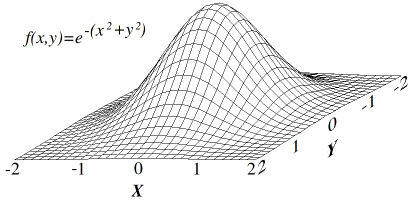
\includegraphics[width=0.6\textwidth,scale=1]{files/Hill_climb.png}  
		\caption{A convex function. Ideal for the hillclimbing method \cite{wiki-hill}.}
		\label{fig:hill}
	\end{figure}
\end{center}

\begin{center}
	\begin{figure}[H]
		\centering
		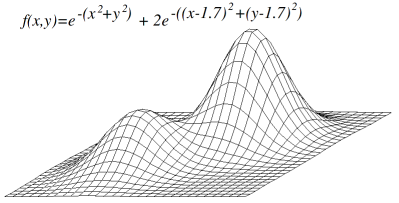
\includegraphics[width=0.6\textwidth,scale=1]{files/Local_maximum.png}  
		\caption{A function with two optima. Hillclimbing could end in the worse optimum if it starts at a bad coordinate. \cite{wiki-hill}.}
		\label{fig:hill2}
	\end{figure}
\end{center}


\subsection{Constraints} %Bedingungen und Nebenbedingungen
The main condition is the fitness-function. Second conditions
can be the

%\subsection{Efficency} %Optional chapter to test the efficency between mathematical methods and evolutionary methods. For example zero of a function.

\section{Variants of the creepy random search method}
In the main-method of the creepy random search you just accept better fitness values after an iteration-step and reject worse ones.
The problem is, that with this algorithm you will mostly get stuck on a local optimum, instead of finding the global one.
To solve this problem you should allow temporal low fitness-values. It should be possible to leave a local optimum to find a better one.
To realise this, there have been developed some extended versions of this method: \\

\fbox{
	\begin{minipage}{15cm}
		\begin{itemize} 
			\item A stagnation of the fitness is allowed by a specified probability (Simulated annealing)
			\item A stagnation of the fitness is allowed till a maximal deterioration. (Threshold accepting, deluge method)
		\end{itemize}
	\end{minipage}
} \\


\subsection{Simulated annealing}
Simulated annealing is a probabilistic optimization method.
It is inspired by the annealing of fluid materia to a solid aggregate states in metallurgy. While cooling down a material the thermodynamic free energy has to get as minimal as possible to get a clear crystalline structure. Therefore its suggested to cool down to material slowly for a better probability of getting a clear solid body.

Analog in optimization you start with a high temperature T, means a big delta, to make wide jumps in the problemphase-space. So jumps between more maxima are possible. At the beginning each chromosome has the same probability to get selected. With each iteration the temperature is reduced and the jumps are getting shorter. Selecting better chromosomes is now more probalistic.
Towards the end the algorithm commutes in a optimum and behaves like the standard hillclimbing-algorithm.

Slowly reducing the temperature increases the chance to find the global optimum. Cooling to fast leads to commuting early into a local optimum instead.

The following formula shows the probability of selecting a chromosome with lower fitness:

\begin{equation}
p(r) = \frac{1}{1+exp(-r/T)}
\end{equation} 

The probability to select a worse chromosome should be small.
At the beginning a big T tends to equalize the probability of all chromosomes. For $T \to \infty$ all chromosomes have the same chance to get selected. Lowering T gives good chromosomes priority. For T = 0.1

\subsection{Threshold accepting}

\section{Recombination}



\section{Applications}
The use of a specific algorithm depends on the problem and its modelisation. In general all optimization-methods are equal in effectivity, if we look over all posible optimization-problems in one set (No-free-Lunch-Theorem Source). Astonishingly a purely random search isn't less effective.
Some of the given methods are better in special cases than others. Also a good understanding of the problems topic is essentially. Evolutinary algortihms take advantage of reducing the set of problems and a good modelisation.
Simulated annealing is suitable for functions with many local optima.

% \section{Genetic algorithms - An artifical duck}

%\chapter{Alternative algorithms}
%In this chapter other intelligent algorithms are presented.
%These algortihms are for comparing the neural network to %simpler
%methods.

%\section{The greedy algorithm}

%\subsection{Weaknesses}

%\section{Applications}





\chapter{The Box2D-Physicsengine}
Box2D is 2-dimensional physics engine, created by Erin Catto. It is licensed under the zlib-license, hence it is noncommercial and open source. The Box2D library is written platform-independently in C++. It is used mainly for gamedevelopment. There exist many portations to other programming languages, like Java and C\#. \\
(source jbox2d)
To setup Box2D look at:
(source http://www.iforce2d.net/b2dtut/setup-linux)

Box2D is used by the project to simulate a realistic physical environment, proving the agents behaviour. \\

Erin Catto wrote a testing gui, called Testbed, using the opengl-framework GLUT, respectively freeglut for windows.

The project-structure is based on the testbed-program.


\section{Core concepts}
In this section the main concepts of Box2D are explained.


\subsection{Bodies}
Bodies are the main objects, affected by physics-simulation.

The body contains the following values: \\

\fbox{
	\begin{minipage}{15cm}
		\begin{multicols}{2}
			\begin{itemize}
			\item \textbf{2D position vector}
			\item \textbf{Angle}
			\item \textbf{Velocity}
			\item \textbf{Angular velocity}
			\item \textbf{rotational inertia}
			\item \textbf{mass}
			\item \textbf{1 or more fixtures}
			\end{itemize}
		\end{multicols}
	\end{minipage}
}   \\
\\



A body contains one or more fixtures, containing the shape and more properties of the body.

If a body is moved, also the fixtures are moved.

\subsubsection*{Bodydefinitions}
To create a body, a bodydefinition has to be created first. It's holding the bodytype, linear- and angular damping values, among other things.
The bodydefinition can also be used to set the start- position and angle of the body. This can increase start-up performance.

\subsubsection*{Body types}
There are three types of bodies:

\fbox{
	\begin{minipage}{15cm}
		\begin{itemize} 
			\item \textbf{Static body}
			\item \textbf{Kinematic body}
			\item \textbf{Dynamic body}
		\end{itemize}
	\end{minipage}
}   \\
\\

A \textbf{static body} is excluded from the simulation. It also doesn't move. Static bodies are used as world-borders for example. Static bodies doesn't collide with other static- or kinematic bodies. \\

A \textbf{kinematic body} can move by setting its velocity, but isn't influenced by forces.
Kinematic bodies doesn't collide with other static- or kinematic bodies.\\

The \textbf{dynamic body} is the commonly used bodytype in Box2D-simulations. It is fully simulated and can be moved by the user or by forces, as its usual way.

\subsubsection*{Damping, friction and gravity scale}
Damping reduces the velocity (linear and angular) of the body.
Friction reduces the velocity of a body at collision with other bodies.

The damping parameter can be zero for no damping and infinite for full damping. In general a value between 0 and 0.1 is used.

The gravity scale is a factor that determines how much the worlds gravity influences the body. 0 determines no influence.

\subsubsection*{Activation and Sleeping}
A body can be set asleep. Sleeping is used to save cpu-time. The body will be woken up, if an other body collides with it.
A body can be completely excluded from simulation by setting it inactive instead.
Instead of the sleeping-mode it will not be woken up.

\subsubsection*{Methods}
TODO

\begin{lstlisting}[caption={Setting body definitions},label=lst:bodydef]
b2BodyDef myBodyDef;
myBodyDef.type = b2_dynamicBody;
myBodyDef.position.Set(0, 20); //set start position
myBodyDef.angle = 0; //set start angle
\end{lstlisting}


Transforming a body
Set Velocity
Set Angular velocity

\subsection{Fixtures}
Fixtures give bodies a shape and additional properties. A body can have multiple fixtures, with their positions relativly to the body's origin.

The following properties are part of a fixture:


\fbox{
	\begin{minipage}{15cm}
	\begin{multicols}{2}
		\begin{itemize} 
			\item \textbf{A shape}
			\item \textbf{Broad-phase proxies}
			\item \textbf{Density}
			\item \textbf{Friction}
			\item \textbf{Restitution}
			\item \textbf{Collision filtering flags}
			\item \textbf{Pointer to the affiliated body}
			\item \textbf{User data}
			\item \textbf{Sensor flag}
		\end{itemize}
	  \end{multicols}
	\end{minipage}
}   \\
\\

A single \textbf{shape} is contained by the fixture. The shape can be a rect, a polygon or a circle. Shapes aren't linked to the body directly, because they may be used independly of the simulation. Therefore the fixture is interposed between body and shape. In Box2D the maximum amount of vertices is defaultly set to eight. A vertex defines the position-vector of an body's edge. A polygon therefore can be created with a minimum of three position-vectors and maximally with eight.
\\

\textbf{Broad-phase proxies} are used internally by Box2D to accelerate collision detection. Therefore a dynamic tree containing the collision-pairs in form of AABB's(footnote) are used. In the most cases it isn't necessary for the user to use proxies. \\

The \textbf{densitiy} is used for computation of the body's mass.\\

The \textbf{friction} of two fixtures is multiplied at collision. \\

\textbf{Restitution} makes a fixture elastic. Usually this value is set between 0 und 1. \\

\textbf{Collision filtering flags} can be used to just allow specified groups of fixtures to collide. \\

A \textbf{pointer to the affiliated body} is stored in the fixture.\\

\textbf{User data} is used as a 'hook' to identify a fixture by an id or add it some self-defined properties. User data is a 'void *'-pointer. Therefore it can contain any datatype. \\

The \textbf{sensor flag} defines that a fixture doesn't interact physically with other fixtures, except by detecting collisions. \\



A fixture is created by initializing a fixture definition and passing its address to the body:

\begin{lstlisting}[caption={Creation of a fixture (source Box2D manual)},label=lst:fixture-create]
b2FixtureDef fixtureDef;
fixtureDef.shape = &myShape;
fixtureDef.density = 1.0f;
b2Fixture* myFixture = myBody->CreateFixture(&fixtureDef);
\end{lstlisting}


\subsection{Joints}
Joints are used to connect two or more bodies. For more detailed information read the Box2D manual Chapter 8.

\subsection{World}
A world is the simulation-environment. It contains all bodies and joints and manages all aspects for simulation. It is the main entity.

The world represents a factory pattern, because it can create and detroy bodies and joints.

\subsubsection*{Simulation parameters}
The physics-simulation is controlled by three parameters: \\

\fbox{
	\begin{minipage}{15cm}
		\begin{itemize} 
			\item \textbf{timeStep} (float32) (Recommended: 1.0f /60.0f respectively 60Hz)
			\item \textbf{velocityIterations} (int32) (Recommended: 8)
			\item \textbf{positionIterations} (int32) (Recommended: 3)
		\end{itemize}
	\end{minipage}
}   \\
\\

These parameters are used by the Step-Method of the world in which one single simulationstep is processed. \\

The \textbf{timeStep} parameter defines the time-resolution on which the simulation will update the environment. A lower timestep improves the quality of the simulation, but on costs of performance. A higher timestep increases the performance, but the simulation can be inaccurate on too low values.
The default value is 60Hz. The author of Box2D suggests not to use values lower than 30Hz. As set, the timestep should not be changed as it could cause unwanted behaviour. For a faster simulation the step-method should just called multiple times. \\


\textbf{Velocityiterations} is the resolution of computing impulses to move bodies precisly. The default value is 8. \\

\textbf{Positioniterations} defines the resolution of overlapping bodies. This is important for a correct collision detection of bodies. The default value is 3. \\


source: www.iforce2d.net/b2dtut/worlds
source: box2d.org/manual.pdf

\subsubsection*{Methods}
TODO
\begin{lstlisting}[caption={World creates a body},label=lst:world-body]
b2Body* m_body = m_world->CreateBody(&myBodyDef);
\end{lstlisting}

\section{Collision detection}
In Box2D collisions are computed between two fixtures. If a collision happens a contact object, containing information about collision coordinates, normals and impulse among ohter things, is created. A contact object can be used to manage a collision.

The collision-computation processes four phases:
TODO: Flowchart of a collision-process:


source: iforce2D


An AABB is an 'axis aligned bounding box'. It completly contains a shape. It is used for fast performance of computing geometrical operations. (source: wikipedia)

\begin{center}
	\begin{figure}[H]
		\centering
		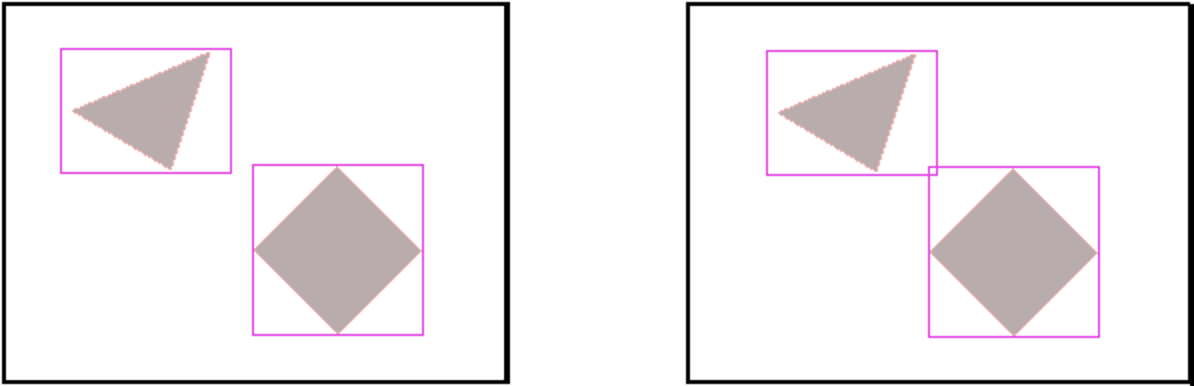
\includegraphics[width=0.8\textwidth,scale=1.0]{files/aabbs-crossing.png}  
		\caption{Two AABBs are overlapping. (source iForce2D) \cite{box2d-iforce}.}
		\label{fig:aabbs}
	\end{figure}
\end{center}
If two AABBs are overlapping, a contact between the two fixtures is created, but the isTouching()-method returns 'False', because the shapes aren't overlapping.

Sometimes, fast moving bodies misses collisions. Therefore it is possible to define the body as a bullet.
This can be accomplished at creation of the body, by the body's definition instance:

\begin{lstlisting}[caption={Define fixture as bullet before creation},label=lst:fixture-bullet-before]
bodyDef.bullet = true;
\end{lstlisting}

Or after the creation of a body by the following method:

\begin{lstlisting}[caption={Define fixture as bullet after creation},label=lst:fixture-bullet-after]
body->SetBullet(true);
\end{lstlisting}

The following figure shows the processing of a collision:

\begin{center}
	\begin{figure}[H]
		\centering
		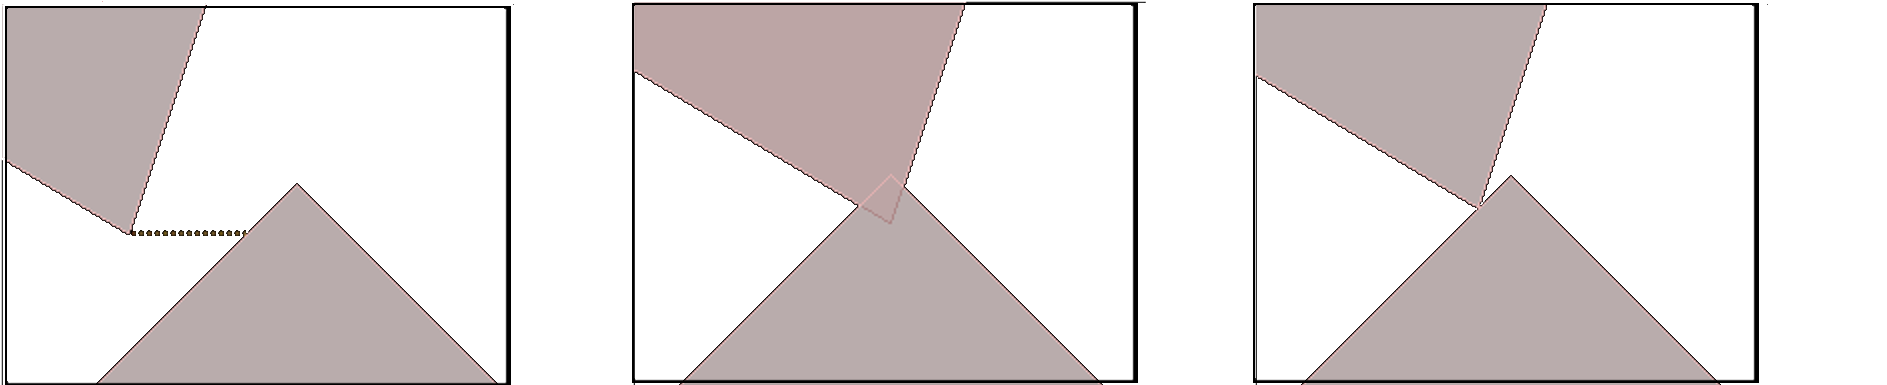
\includegraphics[width=1.0\textwidth,scale=1.0]{files/fixtures-overlap.png}
		\caption{Two fixtures are overlapping (source iForce2D) \cite{box2d-iforce}.}
		\label{fig:fixture-overlap}
	\end{figure}
\end{center}

In the first picture, a contact is created, because the AABBs of the two object are overlapping.
The second picture shows non-bullet bodies overlapping. A bullet-body takes more cpu-time to compute but would get picture three as result.

Bullet bodies

\subsection{Contact listener}
The contact listener calls callback-methods if the events 'Begin contact' and 'End contact' are triggered.
On a collision a contact object is created containing information about the fixtures collision.
Contacts are used to manage collisions between two fixtures.

To access the contact and the two colliding fixture a contact listener should be used.

TODO: accessing contacts, 


\begin{lstlisting}[caption={Contact listener methods},label=lst:collision-contact]
/b2ContactListener
// Called when two fixtures begin to touch
virtual void BeginContact(b2Contact* contact);
// Called when two fixtures cease to touch
virtual void EndContact(b2Contact* contact);
// Called after collision is detected
virtual void PreSolve(b2Contact* contact, const b2Manifold* oldManifold);
// Called after computing the results of the collision
virtual void PostSolve(b2Contact* contact, const b2ContactImpulse* impulse);
\end{lstlisting}

\subsubsection*{Begin contact}
This callback is executed when two fixtures begin touching.

\subsubsection*{End contact}
The end contact callback is called when the two colliding fixtures cease touching.

\subsubsection*{Presolve}
The presolve callback is executed after detection of a collision, but before computing the resulting impulses. It contains a pointer to the contact.

\subsubsection*{Postsolve}
The postsolve callback is executed after computation and applying the contactimpulses of the collision. It contains a pointer to the contact and also the computed impulsedata.

\subsection{Collision filtering}
The default behaviour is that all fixtures can collide with each other. If you want to specify which groups of fixtures can collide and which pass through each other, you can use category- and mask bits to manage 16 groups of fixtures. If you need more precise behaviour you can use group indizes or define own rules by overriding the 'ShouldCollide'-method.

\subsubsection*{Category- and maskbits}

These bits are 16-Bit wide and therefore 16 groups are supported.
Category bits declare on which groups a fixture belongs. A fixture has to belong to minimal one and maximal 16 groups.
The mask bit defines with what group of fixtures this fixture can collide. The default values are 0x0001 for category bits and 0xFFFF for mask bits, meaning every fixture can collide with each other.

\subsubsection*{Group indizes}
Group indizes can be used to get a more specified behaviour as only with category- and maskbits.
The standard value of the group index for a fixture is zero, means group index isn't used, instead the category- and maskbits are used. The value otherwise can be positive or negative.

For a value nonzero the following rules are applied at collision: \\

\fbox{
	\begin{minipage}{15cm}
		\begin{itemize} 
			\item if both groupindizes are different, use the category/mask rules as described above
			\item if both groupindizes are equal and positive, collide
			\item if both groupindizes are equal and negative, don't collide
		\end{itemize}
	\end{minipage}
}   \\
\\

\subsubsection*{Contact filter}
For an own specification of collision behaviour the following virtual method can be overwritten: \\
\begin{lstlisting}[caption={The contact filter method},label=lst:box2d-contactfiler]
bool b2ContactFilter::ShouldCollide(b2Fixture* fixtureA, b2Fixture* fixtureB);
\end{lstlisting}


\section{DebugDraw}
The debugdraw class is used as a debugging feature to display the physics simulation of Box2D. It uses OpenGL. Debugdraw can draw the shapes, contact points, contact normals, the AABBs, etc.
As the debugdraw offers all wanted basic shapes it is used by the simulator.

To use the debug-draw first the debugdraw object hast to be instanciated and linked to the world by: \\

\begin{lstlisting}[caption={Linking debugdraw instance to the world instance},label=lst:box2d-ddrawset]
m_world->setDebugDraw(&m_debugDraw);
\end{lstlisting}

Setting the flags to determine what has to be drawn:

\begin{lstlisting}[caption={Initializing DebugDraw},label=lst:box2d-ddrawinit]
uint32 flags = 0;

flags += b2Draw::e_shapeBit; //Enable drawing shapes
flags += b2Draw::e_jointBit; //Enable drawing joints
flags += b2Draw::e_aabbBit; //Enable drawing AABBs
flags += b2Draw::e_centerOfMassBit; //Enable drawing center of masses

m_debugDraw.SetFlags(flags);
\end{lstlisting}


After each calling of the Step-method the following method has to be called: \\

\begin{lstlisting}[caption={Using debugdraw after each step},label=lst:box2d-ddraw]
m_world->DrawDebugData();
\end{lstlisting}
 
This draws every shape in the bodylist of the world.

\section{Structure of a Box2D-Project}


\begin{center}
	\begin{figure}[H]
		\centering
		\includegraphics[width=0.4\textwidth,scale=0.5]{files/Box2D-structure.png}
		\caption{The general structure of a Box2D-application} \cite{box2d-structure}
		\label{fig:box2d-structure}
	\end{figure}
\end{center}



Important: In BeginContact and EndContact no change of active-flag and some other values of a body/fixture


\section{Testbed}


AnimalFixtureDef[i].isSensor = false;
AnimalFixtureDef[i].friction = 1.0f;
AnimalBodydef[i].linearDamping = 1.0f;
AnimalBodydef[i].angularDamping = 2.0f;

\chapter{The OpenGL graphics library}
OpenGL stands for Open Graphics Library. It is a widely used for developing graphics applications and was published in 1992 by Silicon Graphics. Since 2006 it is maintained by the Khronos Group. It is licensed under a open source license. The logo and the trademark are licensed under a trademark-license.
OpenGL is platform-independent.


It is used by the project to accelerrate the simulator.

The Box2D-Testbed uses GLUT respectively Freeglut and GLUI. Thererefore theses libraries are also used in this project.

source: www.opengl.org
www.sgi.com/tech/opengl/?/

\section{Basics}

\subsection{Cameras}

Model Matrix
Projection Matrix

\section{The OpenGL Utility Toolkit (GLUT)}
The OpenGL Utility Toolkit (GLUT) was developed by Mark Kilgard. It is used to extend OpenGL-Applications by window-management. GLUT is used for small- and medium sized OpenGL-applications.

source: www.codeproject.com/Articles/19760/GLUT-Window-Template

www.opengl.org/resources/libraries/glut/

\subsection{Freeglut}
Freeglut is developed by Pawel W. Olszta and is an alternative to GLUT. It is also a Windows substitute. Freeglut is still maintained. Freeglut is used, because the originally GLUT-library is deprecated and not maintained anymore.

source: freeglut.sourceforge.net/

\subsection{Program structure}
In this section the basic structure of a freeglut-program is explained.
The following code shows the initialization and creation of a window:

\begin{lstlisting}[caption={Initialization a GLUT-program},label=lst:glut-init]
#include "glut.h"

int mainWindow;  //Window handler

int main(int argc, char* argv[])
{
  // Glut initialitation
  glutInit(&argc, argv);
  glutInitDisplayMode(GLUT_RGBA | GLUT_DOUBLE);
  glutInitWindowPosition(0, 0); 
  glutInitWindowSize(1024, 768);
  
  mainWindow = glutCreateWindow("Title");
  
  //Register function callbacks
  glutDisplayFunc(Display);
  glutKeyboardFunc(Keyhandler);
  glutReshapeFunc(Resizehandler);
  
  //Here optionally a GLUI-window can be included, see Chapter 4.3
  
  //Enter glut main loop, usually no return from this function
  glutMainLoop(); 
  return 0;
}
\end{lstlisting}

In the first lines glut is initialised, a window with specified position, size and a title is created.
The variable 'mainWindow' is of type int. It stores the adress of the window-structure.

In the second part of the codesnippet the handler-functions are set. The handler functions have to be static functions, because .
At the end the glut main loop is entered. Usually this function never returns. In Freeglut there exist functions to leave and re-enter the main loop.

The following Codesnippet shows the drawing of a simple triangle:

\begin{lstlisting}[caption={Drawing some graphics},label=lst:glut-draw]
static void Display()
{
  //Set the color to white
  glClearColor(0.0f, 0.0f, 0.0f, 1.0f);
  //Clear the Scene with selected color
  glClear(GL_COLOR_BUFFER_BIT | GL_DEPTH_BUFFER_BIT);
  //Switch to Modelview Matrix
  glMatrixMode(GL_MODELVIEW);
  //Replace the current matrix by the identity matrix
  glLoadIdentity();
  //Draw a blue triangle into the buffer
  glColor3f(0.0f, 0.0f, 1.0f);
  glBegin(GL_TRIANGLES);
  glVertex3f(-0.5f, 0.5f, -5.0f);
  glVertex3f(-1.0f, 1.5f, -5.0f);
  glVertex3f(-1.5f, 0.5f, -5.0f);
  glEnd();
  //Finally draw the scene on screen
  glutSwapBuffers();
}
\end{lstlisting}

The first line sets the draw-color to white and with no transparency. The color is formatted in RGBA. The first three parameters represents the colors red, green and blue. The last parameter is alpha, the transparency of the figure. 0.0f means no quantity of the according parameter and 1.0f as the full quantity.
 This is used by the second line to clear the scene.
Then the viewmode is set, the position of the camera is loaded.
With 'glBegin' the drawing of an object is started. In this example a triangle is drawn. Therefore the three vertices of the triangle has to OpenGl. This is done by. Each object has to finished with the 'glEnd'-command.
At the end the buffer is swapped and the drawn scene is displayed at the screen.

\begin{lstlisting}[caption={Resize camera perspective on window resize},label=lst:glut-resize]
static void Resize(int w, int h)
{
//Set the viewport of the camera
glViewport(0, 0, w, h);
//Switch to the camera perspective matrix
glMatrixMode(GL_PROJECTION); 
//Reset the camera matrix
glLoadIdentity();
//Set camera angle, width-to-height ratio, near z and far z clipping coordinate
gluPerspective(45.0f, (double)w / (double)h, 1.0f, 200.0f);
}
\end{lstlisting}

The first line sets the viewports position and size. The following operations should than applied on the projection-matrix. Therefore the Matrix is resetted to the identity matrix and the clipping of the world the camera should record is set. The near z-coordinate sets the 2D-viewing plane of the camera. The 3D-world will be projected on this 2D-plane. This is the picture that the user will finally see. The far-z perspective defines how deep the sight of the camera into the world is. Objects out of range aren't considered then.
TODO: Figure of the camera perspective

TODO: More Callbacks of GLUT: Idle, etc.

\section{The OpenGL User Interface Library(GLUI)}
The OpenGL User Inteface Library (GLUI) is a GLUT-based user interface library developed by Paul Rademacher. It is written in C++ and usable for multiple platforms.

GLUI is used to implement GUI controls, like buttons, labels, listboxes, etc.

The following figure shows some components of GLUI:

\begin{center}
	\begin{figure}[H]
		\centering
		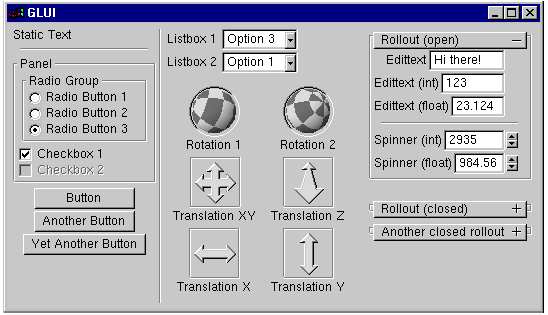
\includegraphics[width=0.8\textwidth,scale=1.0]{files/glui.png}  
		\caption{Some GLUI Components (source www.cs.unc.edu/~rademach/glui/) \cite{ogl-glui}.}
		\label{fig:ogl-glui}
	\end{figure}
\end{center}

source: www.codeproject.com/Articles/20286/GLUI-Window-Template

glui.sourceforge.net/


\subsection{GLUI-Program}

Here is described how a GLUI-window is set up.
The following code is included after the creation of a GLUT-window and before entering the glut main loop (see listing 4.1):


\begin{lstlisting}[caption={Creating a GLUI-window},label=lst:glui-create]
#include "glui.h"
//GLUI window instance
GLUI *glui;

int main(int argc, char* argv[])
{
 ...
 //after creation of glut-window
 glui = GLUI_Master.create_glui("GLUI", 0);
 //Add some components
 glui->add_statictext( "Simple GLUI Example" );
 glui->add_separator();
 glui->add_checkbox( "Wireframe", &wireframe, 1, control_cb );
 GLUI_Spinner *segment_spinner =
 glui->add_spinner( "Segments:",GLUI_SPINNER_INT, &segments );
 segment_spinner->set_int_limits( 3, 60, GLUI_LIMIT_WRAP );
 GLUI_EditText *edittext =
 glui->add_edittext( "Text:", GLUI_EDITTEXT_TEXT, text );
 //Set the main gfx window
 glui->set_main_gfx_window(main_window);
 //Register the Idle callback with GLUI (instead of with GLUT)
 GLUI_Master.set_glutIdleFunc(GlutIdle);
}
\end{lstlisting}

First the glui-instance is initialized. In the following lines gui-components are added. Some components need a variable to point on. This is necessary to store input values from the user. The components can be dimensionized, e.g. the spinners minimum and maximum value is set.
At the end the corrosponding glut window has to be registered in the glui-window.
Callbacks are now defined. This has to be static functions, like in GLUT.

'GLUI\_Master' is a global GLUI-object used to register callbacks, as glui-windows use for example the idle-callback extensively to control components status.

\chapter{Development of a simulator for virtual agents}

\section{Concept}


Transformation of the inputvalues through the input-neurons from range [-20.0, 20.0] and [0.0, 20.0] (Sensor x and y) and [-Pi, +Pi] (DeltaAngle) to the range [-1.0,+1.0] or [0.0, 1.0] with tanh function. (Better function? Linear function?)

Explain why DeltaAngle is necessary:
rotate clockwise. If Agent is rotated by 180degree error should rotate counter-clockwise,but
has learned to rotate clockwise without deltaangle as input.


Optional: Random placment of Objects and agents: see algorithm in NeuralWorld.cpp



Scalability of the World


Modes:
Singleplayer with recording
Supervised learning:
Evolutionary algorithms

Scalable World:
- Size
- Amount of Objects
- Amount of Agents

\section{Software-Engineering}

\subsection{Classdiagram}

\subsection{Use-Cases}

\subsection{The graphical user interface}

Buttons, Modes

Optical Design of the gui

Weight-Matrix

Neural Network Activation

\subsection{The interface}


The inputs: 
x  [0.0, 20.0]
y   [0.0, 20.0]
alpha  [-PI, PI] (Radians)

If no object is detected :
x = 0
y = 0,
alpha = 0 

If an object is detected:
x= Agent.x - Object.x  
y = Agent.y - Object.y
alpha = Agent.Angle - (atan2(det, dot)) 
alpha is the difference between the actual direction of the agent and
the angle between the Position vector of the agent and the object. 
Helpervariables:
determinant: det =  Agent.x * Object.y - Agent.y * Object.x 
dot product:  dot =  Agent.x * Object.x + Agent.y * Object.y 


Outputs are:
Acceleration of the agent: [0.0, 1.0] (with a resolution of 0.001)
multiplied with the maximum accelartion of 
(-sin(Agent->GetAngle())*0.075f * 500 * ,  cos(Agent->GetAngle())*0.075f * 500)

Rotation by angle the agent: [-1.0, 1.0] (with a resolution of 0.001)
multiplied with the maximum rotationspeed of 0.075


\subsection{File saving and loading}

TODO Parser diagram loading the data.

%The
%To minimize  that the agents are missing

\section{OpenGL}
Used to accelerate the simulation.


GLUT, Windows Substitute Freeglut and GLUI. (used because Box2D Testbed used it)

\subsection{Rendering system}

\subsection{ViewPort}

\subsection{MainLoop}

Concept

\subsection{ViewPort}

\section{Box2D}

Call the Step-multiple times instead of changing the timestepvalue

Care that the fixture shapes center is at (0,0) (The body's center). Can be problem at rotation if shape is not centered.

Coordinate system transformation for each agent.

Sensor as semicircle (Source: iforce2D Radarsensor)

Detection of food: atan2-function

\section{Tools}
Make, CMake
Python for Trainingdata

\section{Visualisation}

Fitness Graph
Weight Matrix
Neural Network
% \subsection{The fitness-function}


% \subsection{Neural networks}




\chapter{Results of the simulation}

\chapter{Conclusion}




\KOMAoptions{listof=leveldown}

\newpage

%=========================================LISTS=========================================

\listoffigures
\listoftables
\listofalgorithms
\lstlistoflistings

\newpage

%=========================================DICTIONARY====================================

%dictiary style
\bibliographystyle{./files/alphadin}
%dictionary source
\bibliography{./files/bibdb}


%AI-Junkie Smart Sweepers

%Evolutionäre Algorithmen
%Theorie der neuronalen Netze
%Jonathan Schwarz
%Künstliche Intelligenz

%Box2D Manual
%Box2D Iforce2D

%CMake Manual
%Makefile Manual

%Software-Engineering books?

%Opengl, GLUT and GLUI



\end{document}
